\documentclass[../jb_user_manual.tex]{subfiles}
\begin{document}
%\subsection{How to Use} 
%\subsubsection{Powering things with the JuiceBox}
%When you are powering things with the JuiceBox you have to use power.
\subsection{Charging the JuiceBox}

The juice box should be charged for a minimum of 8 hours following full discharge to restore to full charge.  Draining the batteries frequently and failing to fully recharge them in between uses may contribute to degradation of the batteries, resulting in reduced battery life.

\subsection{Battery Life}

 The juice box can supply up to 16.5 A at 120 VAC.  Battery life is inversely related to current draw; for greater loads, corresponding battery life per charge is reduced.  The graph below shows the relationship between maximum battery life and the percentage of the maximum load.

\vspace{3mm}
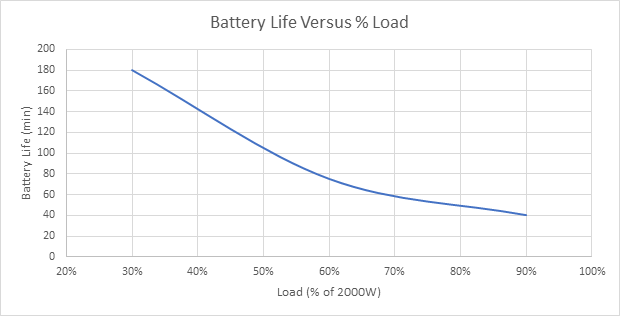
\includegraphics[width=6in]{Battery_Life.png}

Note:  Graph depicts maximum battery life for new unit with fresh batteries at full charge.  Low power alarm will sound before reaching full discharge.


\end{document}